\documentclass[a4paper]{article}

\usepackage[english]{babel}
\usepackage[utf8x]{inputenc}
\usepackage{amsmath}
\usepackage{amsfonts}
\usepackage{graphicx}
\usepackage{subfigure}
\usepackage{url}
\usepackage[colorinlistoftodos]{todonotes}

\title{CS 5785 -- Applied Machine Learning -- Lec.\ 9}
\author{Prof.\ Nathan Kallus, Cornell Tech\\Scribes: Yiren Zhou, Christophe Rimann, Yuemin Niu, Wen Guo}
\date{October 9, 2018}

\begin{document}
\maketitle

\section{Recap}
Inference is essentially opening up the supervised learning ``Black box" in an attempt to understand how $\hat{f}$ depends on data. In the previous lecture, we discussed how inference works for the linear model, as well as confidence intervals for coefficients (i.e. how far we are from where we would be with infinite data).\\


Now, we briefly discuss an aside: standardization and regularization. Recall that the goal of ridge regression is to minimize $$||Y-X\beta||_{2}^2+\lambda\sum_{j=1}^p(\beta_{j})^2$$
If X and Y have different units, the results will not make sense. As such, to make the penalty fair, often we first standardize the data as follows:
$$x_{ij} = \frac{x_{ij}-u_j}{\sigma_j}$$

We do the same for Lasso, given Lasso's dependence on ridge.\newline
This is not an issue for the following: \newline
- Subset selection \newline
- If features are of similar nature e.g. Pixel brightness; word counts 
\newline

\section{Density Estimation}
Consider data $$Y_{1},Y_{2}...Y_{n}\in\mathcal{R}$$ drawn from a distribution with CDF F and PDF f = F'. How do we understand this distribution from data alone? In some sense, how do we estimate F and F?\newline
Estimating F is easy: we can just find the empirical CDF: $$\hat{F}_{n}(y)=\frac{1}{n}\sum_{i=1}^n(\prod(Y_{i}<=y))$$\newline
Estimating f is more difficult. We cannot simply differentiate $\hat{F}$, because it is a stepwise function, which would mean we would have infinite slope at the points where the stepwise function is active, and 0 otherwise. In particular, given $y\not\in Y_{1},Y_{2}...Y_{n}$, we are not sure how dense Y is at y.

\section{Histogram}
One approach is to use histograms. Given a list of cutoffs $$y_{1}<y_{2}<...<y_{n}$$
we can get bins $$[y_{1},y_{2}),[y_{2},y_{3}),...,[y_{n-1},y_{n})$$
From there, we can count how much data is in each bin. $$n_{j}=\sum_{i=1}^n(\prod[Y_{i}\in[y_{j-1},y_{j}]])$$

A histogram is usually just a bar chart with these heights - each bin becomes a bar, with the height being the amount of data in the bin.
How do we choose the bins? Usually segment $[\min Y_{i},\max Y_{i}]$ equally. More sophisticated ways that choose bins automatically are implemented in packages; we will not be covering them in depth.

To make it a density estimate, we need to normalize, so we define a j s.t. $y\in[y_{j-1},y_{j})$
$$\hat{f_{n}}(y) = \frac{n_{j}}{n}\frac{1}{y_{j}-y_{j-1}}$$

There's a problem with this: histograms are not smooth, and don't really look like f? 


\section{Kernel Density Estimation}
Density estimation in general is a key aspect of some supervised learning algorithms we'll be using later on. For now, we are going to use kernel density estimation (a.k.a Parzen Window density estimation) to help solve some of the issues with Histograms, namely their lack of smoothness. Kernel density estimation is essentially a ``smoother" version of a histogram (i.e. a continuous version of a histogram). Analogously, while histograms required us to specify bin widths, we now have to specify a kernel width. 
\\
This is represented as the following equation:
$$\hat{f}_X(x_0)=\frac{1}{N\lambda}\sum_{i=1}^N K_\lambda(x_0, x_i)$$\label
Within this equation, $K_\lambda(x_0, x)=\phi(|x-x_0|/\lambda)$ represents a kernel of width $\lambda$, with center at $x_0$ for a point $x$. $\lambda$ is correspondingly the ``smoothing parameter". We can choose different kernels K (as long as they are non negative functions); one such example and the one used in class is $K_\lambda = \varphi(\frac{u}{\lambda}$, where $\varphi$ is the PDF of the standard Gaussian/Normal distribution: $\varphi(u) = \frac{1}{(2\pi)^{\frac{1}{2}}}e^{-\frac{1}{2}u^2}$. The problem with the Gaussian as shown is that it does not integrate to 1; as such, we divide by $\frac{1}{n\lambda}$ to accommodate for this in the equation for $\hat{f}_X(x_0)$ above.

We can look to figure \ref{fig:systolic} for an example. In this figure, we can see the green ticks representing different levels of systolic blood pressure, where each tick represents one measurement. The blue lines are the kernels formed around each tick: as we can see, we are adding one normal distribution centered around each green tick. The red line is the resulting kernel density estimate, which is formed by summing the kernels at every given point. As such, where the Gaussian functions are more crowded, the kernel density estimate will be larger, while where the Gaussians are more sparse, the kernel density estimate is smaller. 
\begin{figure}
\centering
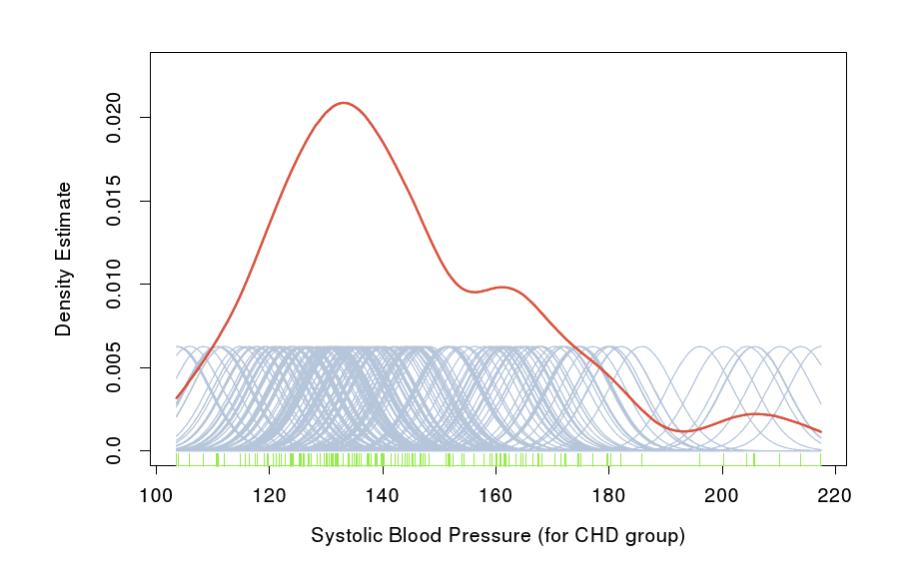
\includegraphics[width=1.0\textwidth]{systolic.png}
\caption{\label{fig:systolic}Systolic blood pressures}
\end{figure}

In figure \ref{fig:kde_2}, we can see the effect of changing $\lambda$s on the resulting KDE. The red line represents a KDE with $\lambda$=0.05, black is 0.337, and green is 2. The grey is the actual true density (the standard normal distribution). We can see that smaller values are rougher, while larger values are smoother. Somewhere in the middle, the grey is fairly close to our true density. In order to establish the correct value for $\lambda$, we will use Cross Validation, with log likelhiood as our loss function.
\begin{figure}
\centering
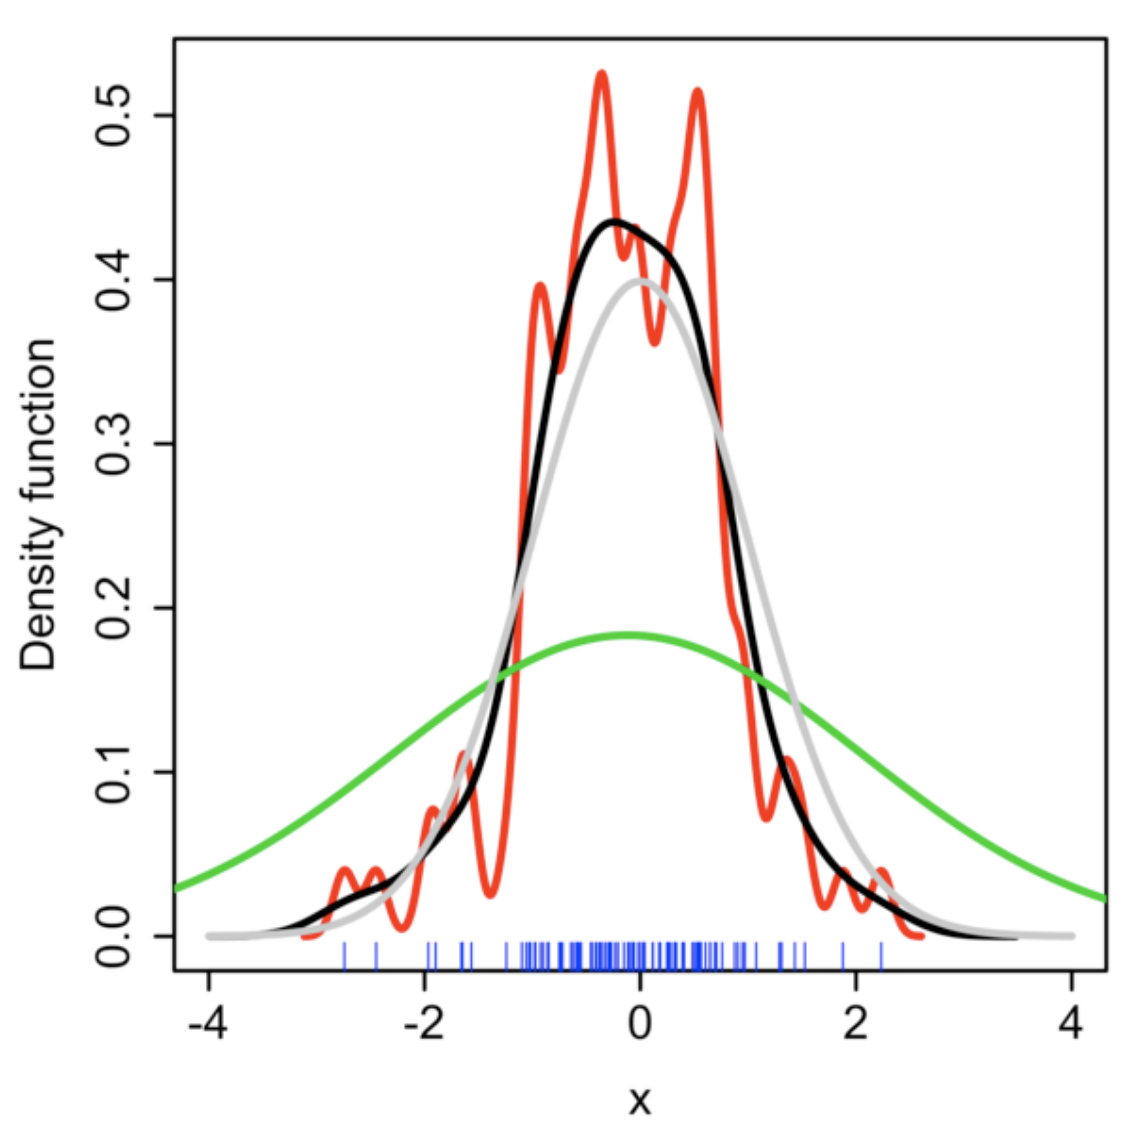
\includegraphics[width=1.0\textwidth]{kde_2.png}
\caption{\label{fig:kde_2}Changing $\lambda$ values for KDE}
\end{figure}

\section{Kernel Regression}
Kernel regression comes from the idea of using weighted average of training data to make prediction. It is actually very similar to k-nearest neighbors regression. However, the exponential weights allow kernel regression to give a continuous and smooth prediction. We can also get the equivalent formula from a kernel density estimation (KDE) perspective. Figure \ref{fig:KNNandKR} shows a comparison between KNN and kernel regression. The KNN prediction is stepwise and discontinous. We can see that kernel regression gives a smooth prediction, which makes it more favorable.
\begin{figure}
\centering
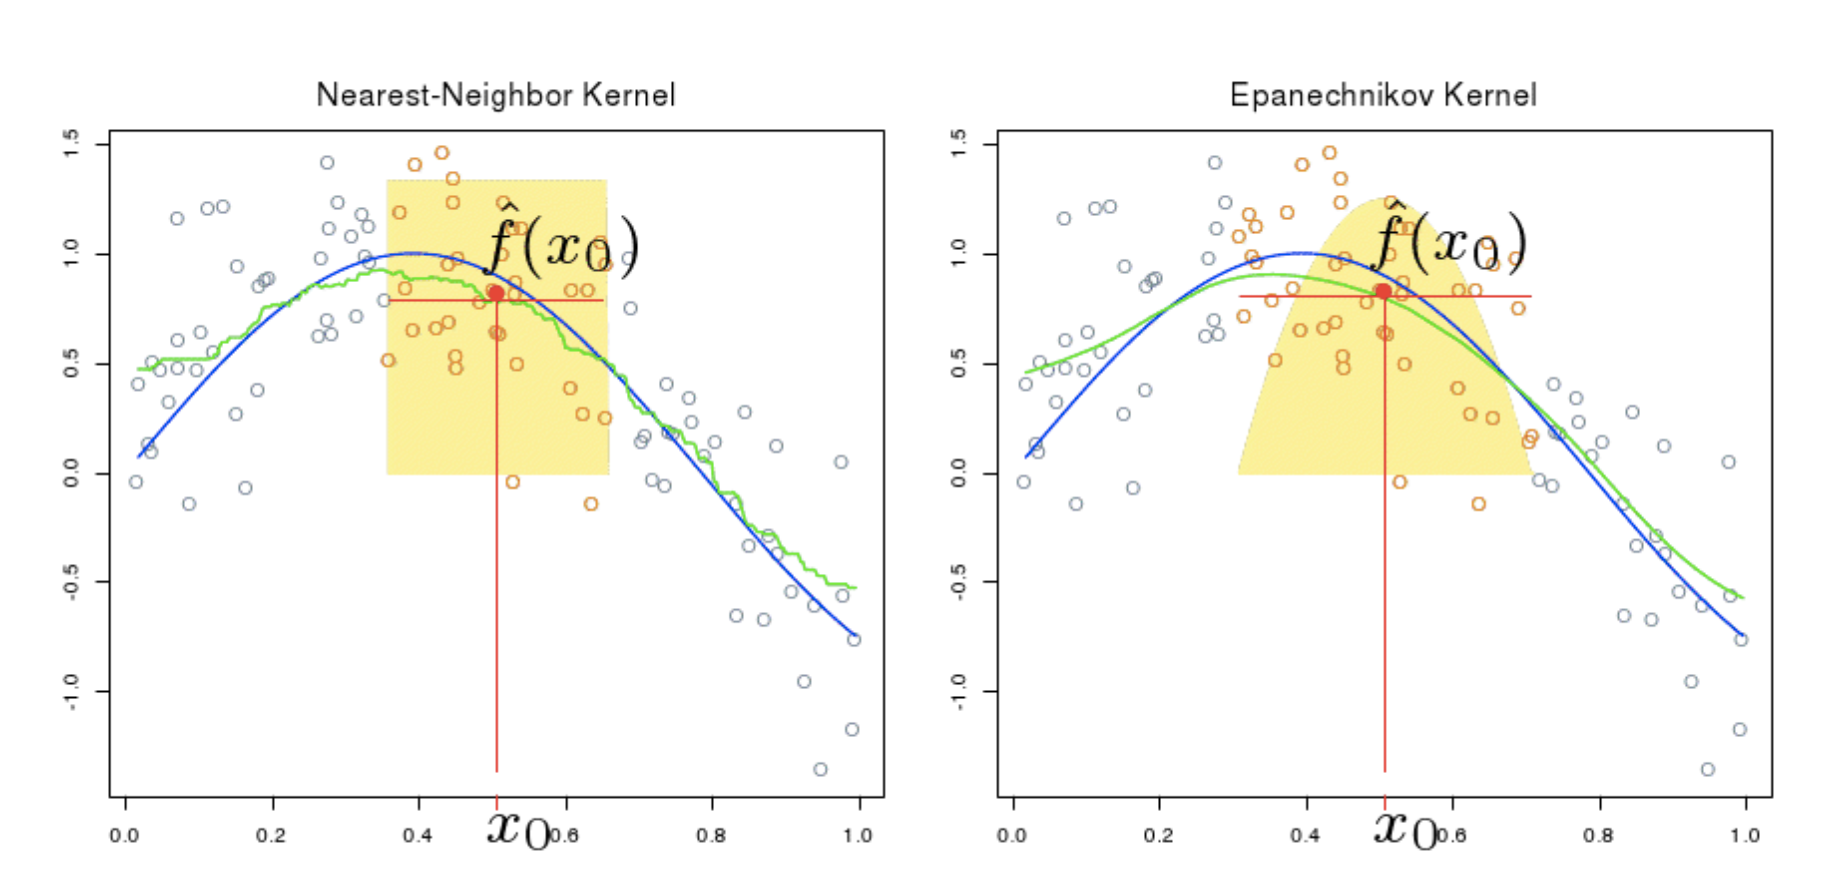
\includegraphics[width=1.0\textwidth]{KNNandKR.png}
\caption{\label{fig:KNNandKR}KNN and Kernel Regression}
\end{figure}

For a regression problem, assume the distribution of $Y$ and $X$ are known. The best prediction for $Y|X=x$ is the conditional expectation:
\begin{align*}
    E[Y|X=x]&=\int yf_{Y|X=x}(y)dy\\
    &=\int y\frac{f_{Y,X}(y,x)}{f_X(x)}dy\\
    &=\frac{\int yf_{Y,X}(y,x)dy}{\int f_{Y,X}(y,x)dy}\\
\end{align*}
However, the joint distribution of $Y$ and $X$, $f_{Y,X}(y,x)$, is unknown and we need to estimate it. If substituted with a kernel density estimation (KDE), we get the kernel regression formulation:
\begin{align*}
    E[Y|X=x]\approx \frac{\int y\hat{f}_{Y,X}(y,x)dy}{\int \hat{f}_{Y,X}(y,x)dy}
\end{align*}
where $\hat{f}_{Y,X}(y,x)$ is substituted by the kernel density estimator for the joint distribution of $(Y, X)$:
\begin{align*}
\hat{f}_{Y,X}(y,x)=\frac{1}{n\lambda}\sum_{i=1}^nK_{\lambda}\left(
\begin{pmatrix}
y \\ x
\end{pmatrix}-
\begin{pmatrix}
Y_i \\ X_i
\end{pmatrix}\right)
\end{align*}
Then the kernel regression estimator $\hat{\mu}_n(x)$ becomes:
\begin{align*}
    \hat{\mu}_n(x)&=\frac{\frac{1}{n\lambda}\sum_{i=1}^n\int y\phi\left(\frac{(y-Y_i)^2+\Vert x-X_i\Vert_2^2}{\lambda}\right)}{\frac{1}{n\lambda}\sum_{i=1}^n\int \phi\left(\frac{(y-Y_i)^2+\Vert x-X_i\Vert_2^2}{\lambda}\right)} \\
    &=\frac{\sum_{i=1}^n\int ye^{-\frac{1}{2\lambda^2}(y-Y_i)^2}e^{-\frac{1}{2\lambda^2}\Vert x-X_i\Vert^2}dy}{\sum_{i=1}^n\int e^{-\frac{1}{2\lambda^2}(y-Y_i)^2}e^{-\frac{1}{2\lambda^2}\Vert x-X_i\Vert^2}dy}\\
    &=\frac{\sum_{i=1}^n K_{\lambda}(x-X_i)\int ye^{-\frac{1}{2\lambda^2}(y-Y_i)^2}dy}{\sum_{i=1}^nK_{\lambda}(x-X_i)\int e^{-\frac{1}{2\lambda^2}(y-Y_i)^2}dy}\\
    &=\frac{\sum_{i=1}^n K_{\lambda}(x-X_i)\int (u+Y_i)e^{-\frac{1}{2\lambda^2}u^2}du}{\sum_{i=1}^nK_{\lambda}(x-X_i)\int e^{-\frac{1}{2\lambda^2}u^2}du}\\
    &=\frac{\sum_{i=1}^n K_{\lambda}(x-X_i)Y_i}{\sum_{i=1}^nK_{\lambda}(x-X_i)}
\end{align*}

We can see from the formula that kernel regression is actually a weighted average for all training points, where every point $(Y_i, X_i)$, $i=1,...,n$ is given weight $\frac{K_{\lambda}(x-X_i)}{\sum_{i=1}^nK_{\lambda}(x-X_i)}$. 

Figure \ref{fig:KR} shows the comparison between different scale parameter $\lambda$. We can see that $\lambda$ acts like the number of neighbors $k$ in KNN, which controls the bias-variance tradeoff. A bigger $\lambda$ puts more weight on local data, and a smaller $\lambda$ smoothes over the whole domain. Figure \ref{fig:Kernels} plots seven different kernels. They all integrate to $1$ and are valid kernels for KDE. The Gaussian kernel is the most commonly used one among them.

\begin{figure}
\centering
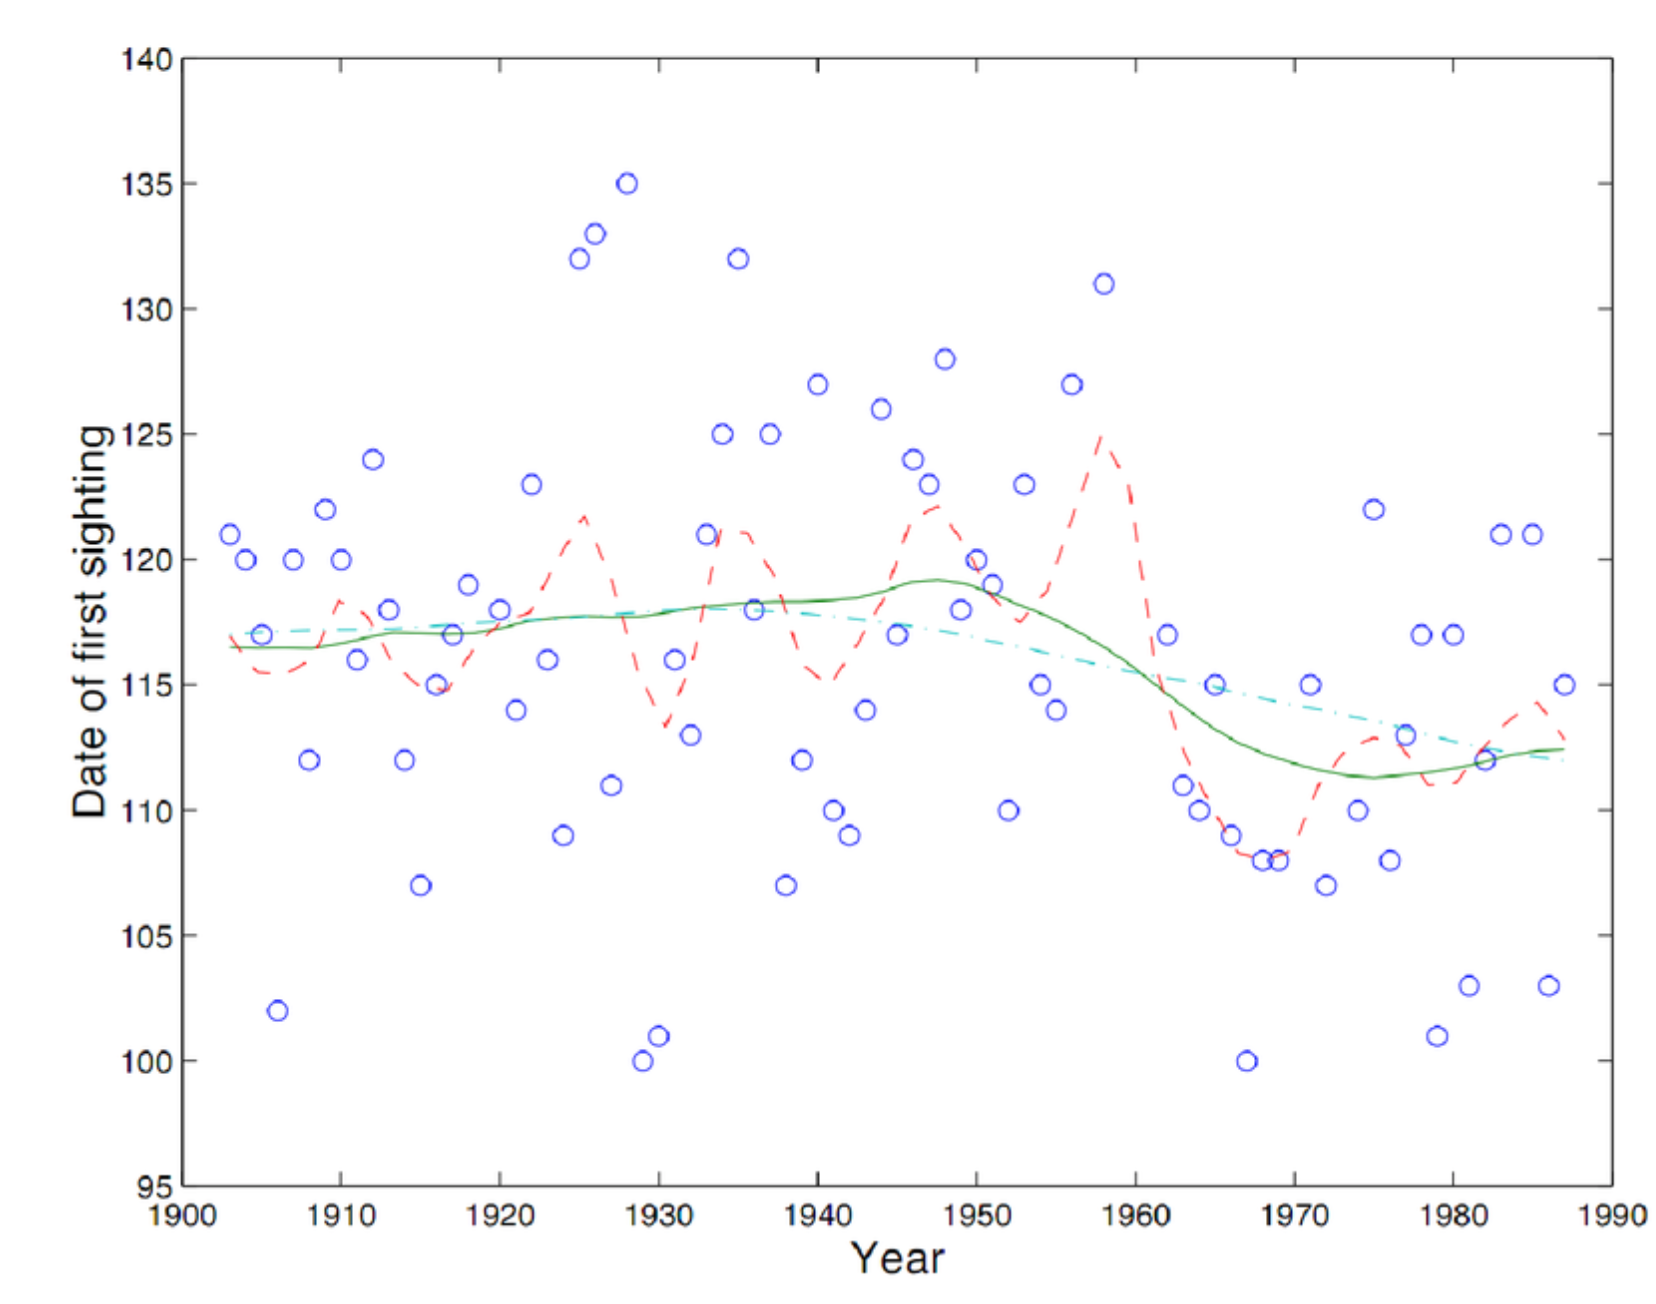
\includegraphics[width=0.9\textwidth]{KR.png}
\caption{\label{fig:KR}Kernel Regression with Different Scale $\lambda$}
\end{figure}
\begin{figure}
\centering
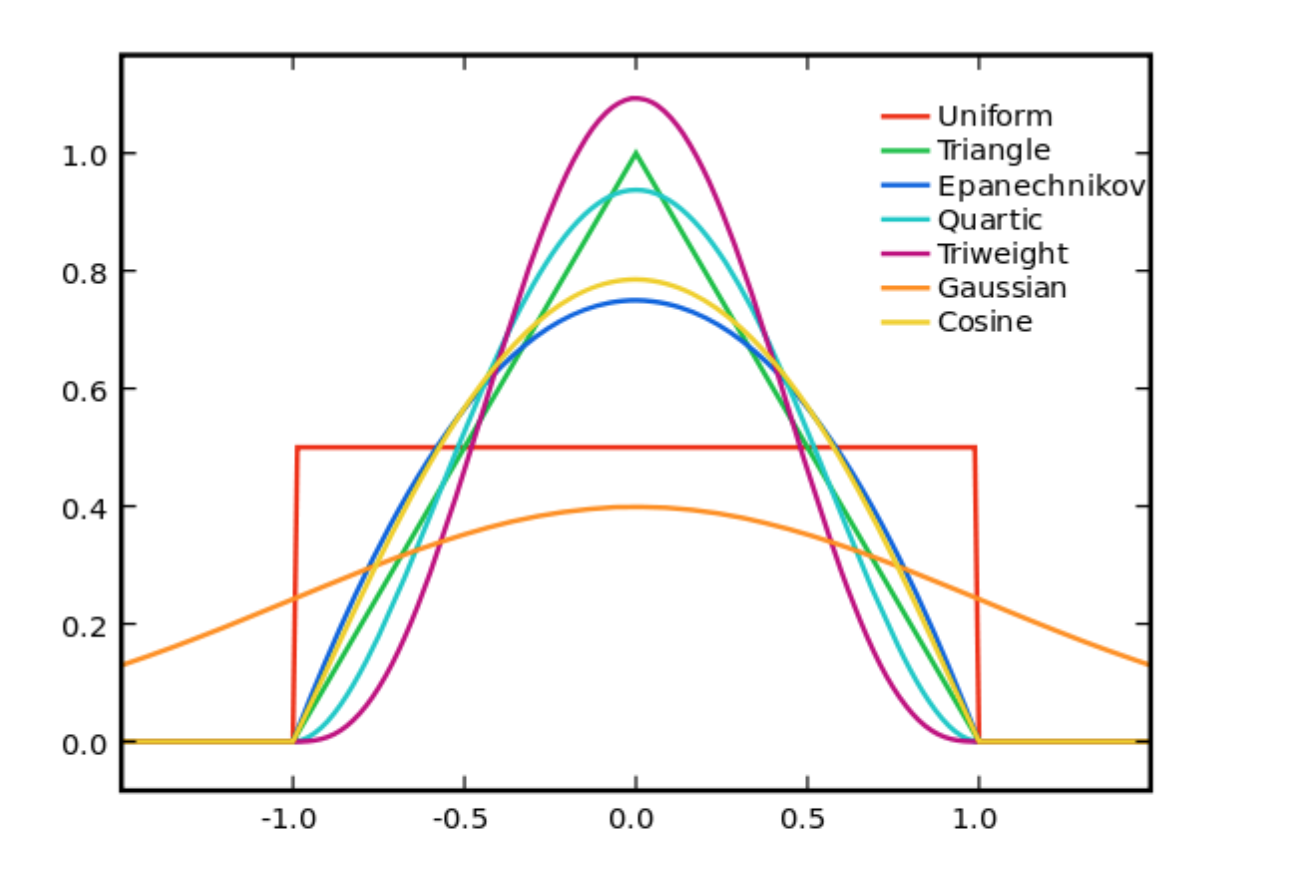
\includegraphics[width=1.0\textwidth]{Kernels.png}
\caption{\label{fig:Kernels}Different Kernels for KDE}
\end{figure}

\section{Kernel Classification}
We can use KDE to obtain classification as well. For instance, let Y be +1 or -1. Then,
$$ P(Y=1|X=x)\geq 0.5 \Longleftrightarrow E[Y|X=x]\geq 0 $$

$$E[Y|X=x] = E[(\prod[Y=1]-\prod[Y\neq 1])|X=x] $$
From here, we can apply the kernel regression to estimate E[Y|X=x] and apply this estimate.

%$$ P(Y=1|X=x)-P(Y\neq1|X=x) $$%

$$\hat\mu(x) \geq 0 \Longleftrightarrow  \frac{1}{n\lambda}\sum_{i=1}^n K_{\lambda} (x-x_{i})y_{i} \geq 0 $$

$$\frac{1}{n\lambda}\sum_{Y_{i}=+1} K_{\lambda} (x-x_{i}) \geq  \frac{1}{n\lambda}\sum_{Y_{i}=-1} K_{\lambda} (x-x_{i})   $$
$$\frac{n_{1}}{n}\frac{1}{n_{1}\lambda}\sum_{Y_{i}=+1} K_{\lambda} (x-x_{i}) \geq  \frac{n_{-1}}{n}\frac{1}{n_{-1}\lambda}\sum_{Y_{i}=-1} K_{\lambda} (x-x_{i})   $$
where $n_1$ is the number of positive examples. Applying the KDE of x among positive examples $\hat f$, we get:
$$\hat\pi_1\hat f_1(x) \geq \hat\pi_{-1}\hat f_{-1}(x) $$
By rearranging terms and apply logs, we can obtain the kernel estimated log odds:
$$log\frac{\hat\pi_1}{\hat\pi_{-1}} + \frac{log\hat f_1(x)}{log\hat f_{-1}(x)} \geq 0$$
Rather than just allowing Y to take on values of + or - 1, we can generalize this classification beyond two possible values with the following:
$$\hat P(Y=j | X=x) = \frac{\hat\pi_j\hat f_j(x)}{\sum_{k=1}^m\hat\pi_k \hat f_k(x)}$$

We can see that as dimensions grow bigger, equivalent sized boxes cover less data.
\end{document}
